% !TEX root = main.tex

\section{线性模型}
线性模型
\[f(\vx)=\vw^\T\vx+\vb\]
由于$\vw$直观表达了各属性在预测中的重要性,因此线性模型具有很好的可解释性(comprehensibility)。

\subsection{线性回归}
数据集$D=\{(\vx_i,y_i\}_{i=1}^m$,每个样本$\vx_i$都由$d$个属性描述,多元线性回归希望(multivariate linear regression)学到
\[f(\vx_i)=\vw^\T\vx_i+b,\;s.t.\,f(\vx_i)\simeq y_i\]

将$\vw$和$b$写在一起变成$\vw\gets\bmat{\vw & b}$,并设
\[X=\bmat{x_{11} & x_{12} & \cdots & x_{1d} & 1\\x_{21} & x_{22} & \cdots & x_{2d} & 1\\
\vdots & \vdots & \ddots & \vdots & \vdots\\x_{m1} & x_{m2} & \cdots & x_{md} & 1}=\bmat{\vx_1^\T & 1\\\vx_2^\T & 1\\\vdots & \vdots\\\vx^\T_m & 1}\]
为已知,$\vw$为需要训练的权重。
再将标记写成向量形式$\vy=\bmat{y_1 & y_2 &\cdots & y_m}$,进而得到最小二乘优化
\[\vw^\star=\argmin_\vw\norm{\vy-X\vw}_2^2\]

对$\vw$求导有
\[\nabla_\vw E_\vw=2X^\T(X\vw-\vy)\]
当$X^\T X$满秩或正定时,令上式为0有
\[\vw^\star=(X^\T X)^{-1} X^\T\vy\]
但现实中大多数时候$X^\T X$都非可逆阵,故常用正则化方法。

\subsection{线性分类}
单位阶跃(unit-step)函数
\[y=\begin{cases}
0 & z<0\\
0.5 & z=0\\
1 & z>1
\end{cases}\]
不连续,故用对数几率(logistic)函数替代
\[y=\frac{1}{1+\ee^{-z}}\]
这是一种Sigmoid函数,将线性表达式代入有
\[y=\frac{1}{1+\ee^{-(\vw^T\vx+b)}}\]
进而有
\[\vw^\T\vx+b=\ln\frac{y}{1-y}\]
将$y$视为样本$\vx$为正例的可能性,则$1-y$为反例可能性,两者比值$y/(1-y)$称为几率(odds),反映了$\vx$作为正例的相对可能性。
对数几率又称logit,故这种方法又称为逻辑斯蒂(logistic)回归,但其实是分类学习方法,是一种\textbf{广义的线性模型}。

优点:无须事先假设数据分布,可以得到类别的近似概率预测,可直接应用现有的数值优化算法求得最优解。

将$y$视为后验概率估计,有
\[\ln\frac{\prc{y=1}{\vx}}{\prc{y=0}{\vx}}=\vw^\T\vx+b\]
显然有
\[\begin{aligned}
\prc{y=1}{\vx}&=\frac{\ee^{\vw^\T+b}}{1+\ee^{\vw^\T\vx+b}}\\
\prc{y=0}{\vx}&=\frac{1}{1+\ee^{\vw^\T\vx+b}}
\end{aligned}\]

给定数据集$\{(\vx_i,y_i)\}_{i=1}^m$,由极大似然法估计$\vw$和$b$有
\[\ell(\vw,b)=\sum_{i=1}^m\ln\prc{y_i}{\vx_i;\,\vw,b}\]

可以用梯度下降或牛顿法进行求解。

\subsection{线性判别分析}
线性判别分析(Linear Discriminant Analysis, LDA)[Fisher, 1936]同样用于二分类,希望将样例投影到一条直线上,使得\textbf{同类样例投影点尽可能近,异类样例投影点尽可能远}。
可通过\textbf{同类样例投影点协方差尽可能小},\textbf{异类样例类中心距离尽可能大}实现。
\begin{figure}[H]
\centering
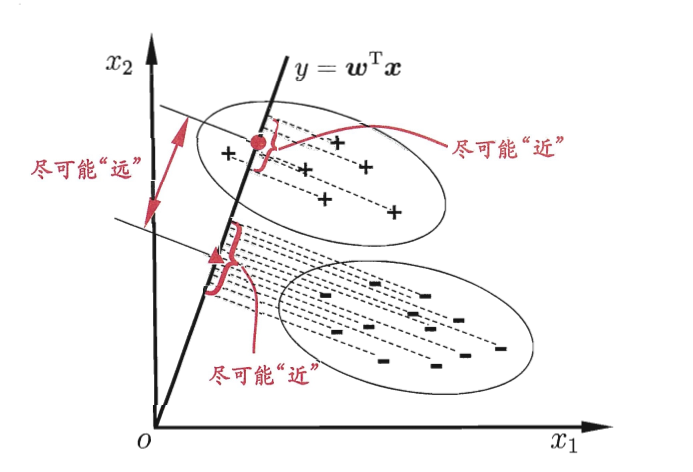
\includegraphics[width=0.5\linewidth]{fig/LDA.png}
\end{figure}

最优化广义瑞利商
\[\begin{aligned}
J &= \frac{\vw^\T(\vmu_0-\vmu_1)(\vmu_0-\vmu_1)^\T\vw}{\vw^\T(\Sigma_0+\Sigma_1)\vw}\\
&= \frac{\vw^\T S_b\vw}{\vw^\T S_w\vw}
\end{aligned}\]
其中$S_w$为类内散度矩阵,$S_b$为类间散度矩阵。
\[\begin{aligned}
S_w &= \Sigma_0 + \Sigma_1\\
&= \sum_{\vx\in X_0}(\vx-\vmu_0)(\vx-\vmu_0)^\T
+ \sum_{\vx\in X_1}(\vx-\vmu_1)(\vx-\vmu_1)^\T\\
S_b &= (\vmu_0-\vmu_1)(\vmu_0-\vmu_1)^\T
\end{aligned}\]

LDA也是经典的监督降维技术。

\subsection{多分类学习}
利用二分类学习器解决多分类问题,拆分策略:
\begin{itemize}
	\item 一对一(One vs. One, OvO):共$\binom{n}{2}=n(n-1)/2$个学习器,\textbf{投票}产生最终结果
	\item 一对其余(One vs. Rest, OvR):一类作为正例,其他作为反例,$n$个学习器,\textbf{置信度最大}的作为最终类别
	\item 多对多(Many vs. Many, MvM)
\end{itemize}

\subsection{类别不平衡问题}
\begin{itemize}
	\item 欠采样(undersampling):减少样例
	\item 过采样(oversampling):增加样例
	\item 阈值移动(threshold-moving)/再缩放(rescaling)
	\[\frac{y'}{1-y'}=\frac{y}{1-y}\times\frac{m^-}{m^+}\]
\end{itemize}